\documentclass[tikz]{standalone}
\usepackage{pgfplots}
\pgfplotsset{compat=1.15}
\usepackage{mathrsfs}
\usetikzlibrary{arrows,calc}
\usepackage{tkz-euclide}
\pagestyle{empty}

\definecolor{AngleClr}{rgb}{0,0.39215686274509803,0}
\definecolor{ShapeClr}{rgb}{0.6,0.2,0}
\definecolor{BlueSqr}{RGB}{5,81,163}
\definecolor{RedSqr}{RGB}{0, 156, 0}

\begin{document}

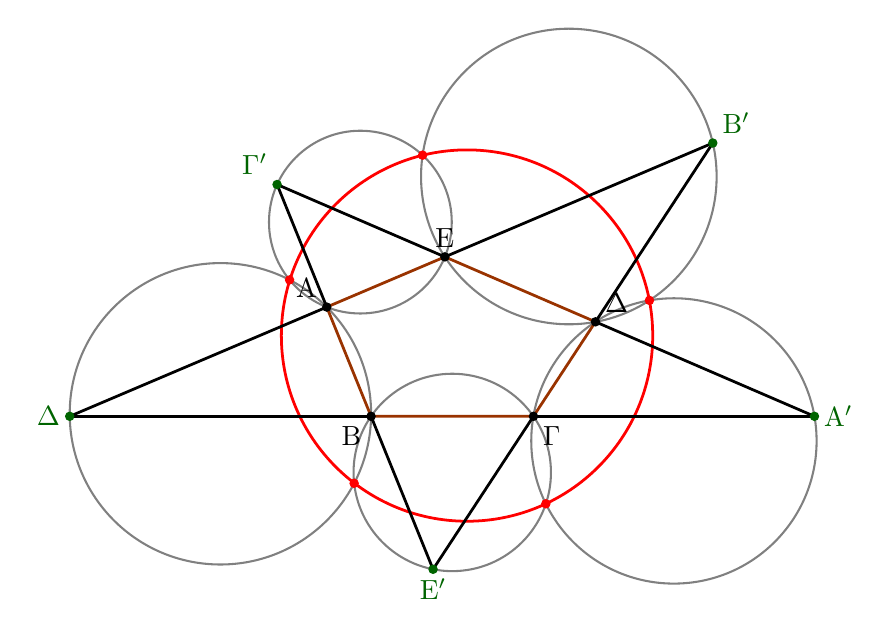
\begin{tikzpicture}[scale=.75]
\tkzSetUpLine[line width=1pt,color=black]
\tkzSetUpPoint[fill=black]

\tkzDefPoints{0/0/B,2.75/0/C,-0.75/1.85/A,1.25/2.7/E,3.8/1.6/D}

\tkzInterLL(A,B)(C,D) \tkzGetPoint{A1}
\tkzInterLL(B,C)(D,E) \tkzGetPoint{A2}
\tkzInterLL(C,D)(E,A) \tkzGetPoint{A3}
\tkzInterLL(D,E)(A,B) \tkzGetPoint{A4}
\tkzInterLL(E,A)(B,C) \tkzGetPoint{A5}

\tkzDefCircle[circum](A1,B,C) \tkzGetPoint{O1}
\tkzDefCircle[circum](A2,C,D) \tkzGetPoint{O2}
\tkzDefCircle[circum](A3,D,E) \tkzGetPoint{O3}
\tkzDefCircle[circum](A4,E,A) \tkzGetPoint{O4}
\tkzDefCircle[circum](A5,A,B) \tkzGetPoint{O5}

\tkzInterCC(O1,A1)(O2,A2) \tkzGetPoints{x}{B1}
\tkzInterCC(O2,A2)(O3,A3) \tkzGetPoints{x}{B2}
\tkzInterCC(O3,A3)(O4,A4) \tkzGetPoints{x}{B3}
\tkzInterCC(O4,A4)(O5,A5) \tkzGetPoints{x}{B4}
\tkzInterCC(O5,A5)(O1,A1) \tkzGetPoints{x}{B5}

\tkzDefCircle[circum](B1,B2,B3) \tkzGetPoint{O}


\tkzFillPolygon[fill=white](A,B,C,D,E)

\tkzDrawCircle[line width=0.75pt](O1,A1)
\tkzDrawCircle[line width=0.75pt](O2,A2)
\tkzDrawCircle[line width=0.75pt](O3,A3)
\tkzDrawCircle[line width=0.75pt](O4,A4)
\tkzDrawCircle[line width=0.75pt](O5,A5)

\tkzDrawCircle[red,line width=1.0pt](O,B1)

\tkzDrawSegments(A1,B A1,C)
\tkzDrawSegments(A2,C A2,D)
\tkzDrawSegments(A3,D A3,E)
\tkzDrawSegments(A4,E A4,A)
\tkzDrawSegments(A5,A A5,B)

\tkzDrawPolygon[color=ShapeClr](A,B,C,D,E)
\tkzDrawPoints[size=3](A,B,C,D,E)
\tkzDrawPoints[size=3,AngleClr](A1,A2,A3,A4,A5)
\tkzDrawPoints[size=3,red](B1,B2,B3,B4,B5)

\tkzLabelPoint[above left](A){$\mathrm{A}$}
\tkzLabelPoint[below left](B){$\rm B$}
\tkzLabelPoint[below right](C){$\rm \Gamma$}
\tkzLabelPoint[above right](D){$\rm \Delta$}
\tkzLabelPoint[above](E){$\rm E$}

\tkzLabelPoint[below,AngleClr](A1){$\rm E'$}
\tkzLabelPoint[right,AngleClr](A2){$\rm A'$}
\tkzLabelPoint[above right,AngleClr](A3){$\rm B'$}
\tkzLabelPoint[above left,AngleClr](A4){$\rm \Gamma'$}
\tkzLabelPoint[left,AngleClr](A5){$\rm \Delta$}

\end{tikzpicture}

\end{document}
